\section{Abtastung}\label{3}
Wird ein Vorgang zu (in der Regel) äquidistanten Zeitpunkten gemessen, so bezeichnet sich dies als Abtastung. Dies ist ein fundamentaler und in der Regel der erste Schritt für die Verarbeitung eines Signals. Im Folgenden werden zunächst die Grundlagen und die Theorie der Abtastung erörtert. Anschließend werden die wichtigsten Eigenschaften aufgezählt und bewiesen. In Abschnitt \ref{3.3} wird auf die Bedeutung dieser Eigenschaften im Kontext eines DSPs eingegangen. Zuletzt wird die Realisierung der Abtastung am Beispiel eines DSPs beschrieben, wobei Fokus auf die Problematiken und Lösungen gelegt wird.
\subsection{Theorie}\label{3.1}
Für jegliche Verarbeitung mithilfe eines DSPs, zur Übertragung mittels beispielsweise des 'Digital Audio Broadcastings' oder zur Minimierung des Speicherverbrauchs ist die Digitalisierung ein notwendiger Schritt in der Signalverarbeitung. 

\subsubsection{Analoge/Digitale Definitions- und Wertebereiche}
%\begin{figure}
%\centering
%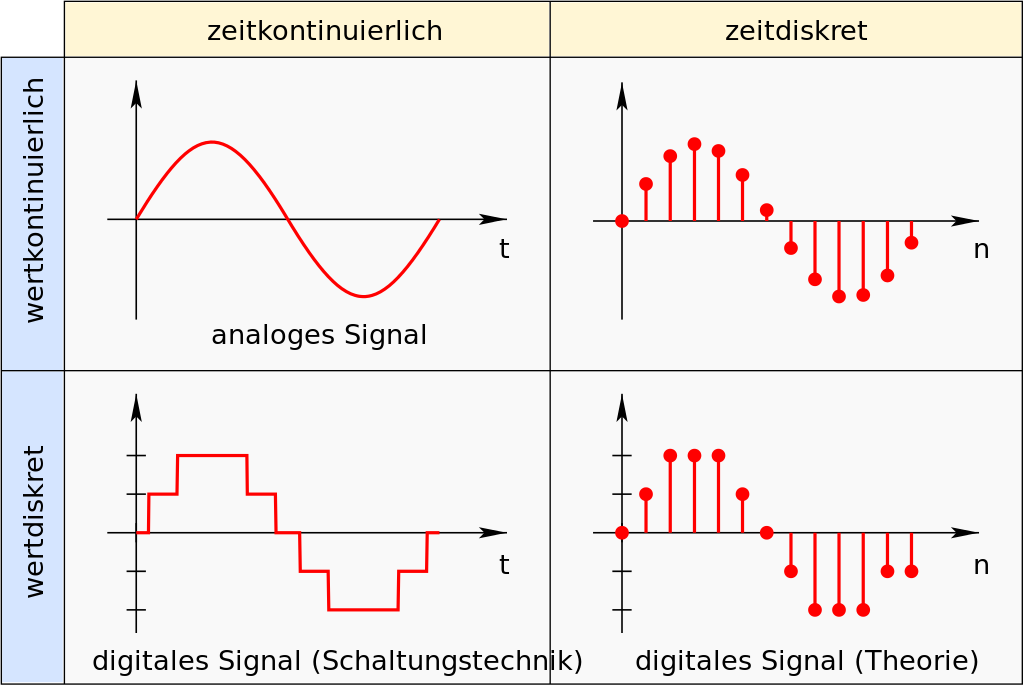
\includegraphics[scale=0.4]{images/signals.png}
%\captionsource{Übersicht diskreter und kontinuierlicher Signale}{\cite[p. 2]{frey2008signal}}
%\label{signals}
%\end{figure}
Grundlegend existieren vier Formen, in denen ein Signal vorliegen kann. Dies wird in \ref{signals} dargestellt. Sowohl im zeit- als auch im Wertebereich können Datenpunkte in diskreter- sowie kontinuierlicher Form vorliegen. Geht man von einer rein kontinuierlicher Form der natürlich existierenden Werte aus, beispielsweise akustische Signale oder auch Temperatur, so besitzen all diese Signale eine zeit- als auch wertkontinuierliche Form.\\
Es existieren Ansätze in der Physik, nach welchen Zeit oder auch Distanz ein rein diskretes Konstrukt beschreiben, da diese eine beliebig kleine, jedoch konstante minimale Einheit besitzen. Auf diese Fragestellung wird hier jedoch nicht eingegangen, und somit wird angenommen, dass ein kontinuierlicher Zeitbereich existieren kann.\\
\newpage

\subsubsection{Ideale Abtastung}
\begin{definition}{Abtastrate}\\
Wird ein Signal im gleichmäßigem Abstand $T_A$ erfasst, so beschreibt $f_A = \frac{1}{T_A}$ die Abtastfrequenz. Der n-te Wert liegt bei $t = n \cdot T_A$ vor.
\end{definition}

Bei der idealen Abtastung wird ein Dirac-Kamm, also eine Folge von Dirac-Stößen $\delta(t)$ genutzt. Liegt nun ein Signal $s(t)$ vor, so ergibt sich das abgetastete Signal wie folgt:\\
$$s_a(t) = s(t) \cdot \sum_{n=-\infty}^{\infty} \delta(t - nT_A)$$\\

\begin{figure}[h!]
\centering
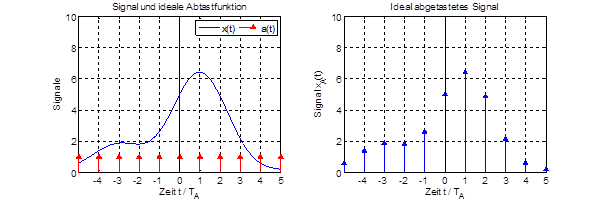
\includegraphics[scale=1]{images/abtastung_ideal.png}
\captionsource{Reale Abtastung eines Signals}{\cite{ideal_abtastung}}
\label{ideal_abtastung}
\end{figure}


Dies ist jedoch lediglich ein mathematisches Konstrukt, und in der Anwendung kann dieses nicht genutzt werden. Im Folgenden wird die reale Abtastung behandelt.

\subsubsection{Reale Abtastung}
In der Realität existieren keine idealen Dirac-Stöße, da diese unendlich steile Flanken besitzen würden. Anstelle des Dirac-Kamms wird eine periodische Folge von Rechteckimpulsen gewählt. Diese wird wie folgt beschrieben:\\
\begin{equation}
   rect(t) =
   \begin{cases}
     0 & ,|t| > \frac{1}{2}\\
     \frac{1}{2} & ,|t| = \frac{1}{2}\\
     1 & ,|t| < \frac{1}{2}\\
   \end{cases}
\end{equation}

Genau wie der Dirac-Impuls besitzt auch die Rechteckfunktion zwei unendlich steile Flanken, die dessen optimale Implementierung unmöglich machen. Jedoch sind hier steigende- und fallende Flanke durch die Dauer $T_W$ getrennt. Dies entspricht der Breite des Rechtecks. Zudem ist eine Flankendauer $T_F$  um einiges irrelevanter, da diese hier nur einen Bruchteil der Funktion ausmacht ($\frac{T_F}{T_W + T_F}$). \\
\newline
Zu einem beliebigen Zeitpunkt $t$ ergibt sich der Abtastwert:\\
$$s_{AW}(t) = \sum_{n=-\infty}^{\infty} s(n\cdot T_A) \cdot rect\left( \frac{t - n \cdot T_A}{T_W}\right) dt 
= rect\left(\frac{t}{T_W}\right) * \sum_{n=-\infty}^{\infty} s(t) \delta (t - n\cdot T_A)$$ \\
Dabei stellt $*$ den Faltungsoperator dar.

\begin{figure}[h!]
\centering
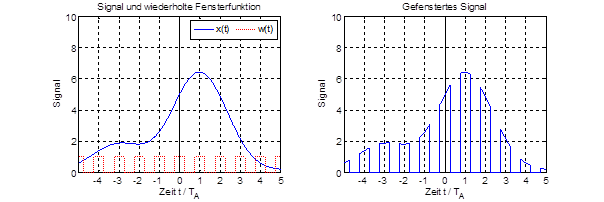
\includegraphics[scale=1]{images/abtastung_real.png}
\captionsource{Reale Abtastung eines Signals mit $T_A = 0.5\cdot T_W$}{\cite{real_abtastung}}
\label{real_abtastung}
\end{figure}

Innerhalb der Zeit $T_W$ wird das eingehende Signal erfasst und integriert, um so einen Wert zu bestimmen. Anschließend wird dieser Wert als konstant angenommen, bis die nächste Periode beginnt. 

\begin{figure}[h!]
\centering
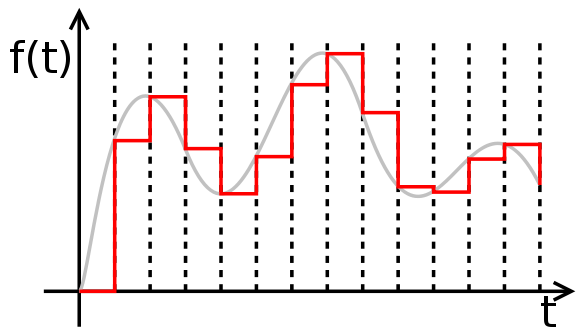
\includegraphics[scale=0.4]{images/sah_signal.png}
\captionsource{Abtastung eines Signals. Die vertikalen, gestrichelten Linien stellen den kaum sichtbaren Zeitraum $T_W$ dar.}{\cite{sah_signal}}
\label{sah_signal}
\end{figure}

\subsubsection{Nyquist-Shannon-Abtasttheorem}
Im Jahr 1948 formulierte Claude E. Shannon ein Theorem, welches einer abzutastenden Funktion $s(t)$ eine minimale Abtastfrequenz $f_A$ zuordnet.\\
Ist das Signal $s(t)$ bandbegrenzt und besitzt eine maximale Frequenz $f_{max}$, so muss die Abtastfrequenz $f_A \geq 2 \cdot f_{max}$ betragen. Ein Beweis folgt in \ref{3.2}.\\
Wird eine geringere Abtastfrequenz gewählt, so kann dies zu Aliasing führen. Somit wird es unmöglich, das originale Signal aus den vorliegenden Informationen zu rekonstruieren, und es liegt Informationsverlust vor.\\
Wählt man eine höhere Frequenz, so gewinnt man keine zusätzlichen Informationen. Allerdings wird das Verfahren robuster, da die von dem Theorem beschriebene minimale Abtastfrequenz nur in einem idealen System zutrifft. In einem realen System existieren beispielsweise keine idealen Filter, da keine unendlich steilen Flanken realisierbar sind. Dadurch würde eine Abtastfrequenz von $f_A = 2 \cdot f_{max}$ ebenfalls zu Aliasing führen.\\
Aus diesem Grund existiert in der Praxis folgender Richtwert:\\
$$f_A \geq 2.2 \cdot f_{max}$$


\subsubsection{Quantisierung}
Im Wertebereich wird das Verfahren der Diskretisierung als 'Quantisierung' bezeichnet. Dies ist zunächst keine Form der Abtastung, ist jedoch eng mit dieser verwandt und wird somit kurz beschrieben.\\

Zunächst wird eine Auflösung $\delta$ gewählt, welche die Ordinate in äquidistante 'Stufen' einteilt. Jeder gemessene Wert wird zur Speicherung einer dieser Stufen zugeordnet, wobei in der Regel die Stufe mit dem geringsten Abstand zu dem Wert gewählt wird. Ein gemessener Wert $x$ wird mithilfe der im Folgenden beschriebenen Funktion einer Stufe zugeordnet.\\
$$Q(x) = sgn(x) \cdot \delta \cdot \Big\lfloor \cfrac{|x|}{\delta} + \cfrac{1}{2} \Big\rfloor $$\\
Hierbei beschreibt $sgn$ die Signum Funktion.\\
Für einen Wertebereich der Größe $l$ ergeben sich $N = \cfrac{l}{\delta}$ Stufen, welcher ein gemessener Wert zugeordnet werden kann. Es ist offensichtlich, dass mit einer genaueren (kleineren) Auflösung eine höhere Genauigkeit erzielt werden kann. Hierzu muss jedoch eine höhere Datenrate in Kauf genommen werten.


\subsection{Mathematische Hintergründe}\label{3.2}
Im Folgenden werden Herleitungen und Beweise zu den in \ref{3.1} erwähnten Theoremen aufgeführt.

\subsubsection{Ideale Abtastung}
Gegeben sei das abgetastete Signal\\
$$s_a(t) = s(t) \cdot \sum_{n=-\infty}^{\infty} \delta(t - nT_A)$$\\
$\mathcal{F}$ bezeichne im Folgenden die Fouriertransformation eines Signals. Es ergibt sich:\\
\begin{equation}
\begin{aligned}
\mathcal{F}(s_a(t)) = &  \mathcal{F}(s(t) \cdot \sum\limits_{n=-\infty}^{\infty} \delta(t - nT_A)) \\
= & \mathcal{F}(s(t)) \cdot \mathcal{F}(\sum\limits_{n=-\infty}^{\infty} \delta(t - nT_A))) \\
= & S(f) * \left[ \frac{1}{T_A} \sum_{n = -\infty} ^ {\infty} \delta \left( f - \frac{n}{T} \right) \right] \\
= & \frac{1}{T_A} \sum_{n = -\infty} ^ {\infty} S\left( f - \frac{n}{T_A} \right)
\end{aligned}
\end{equation}



Es ergibt sich eine periodische Folge des Spektrums von $s(t)$ in einem Abstand von $T_A$. Ist $s(t)$ von einer Frequenz $f_{max}$ bandbegrenzt, wobei $$2f_{max} = f_A $$ 
so ergibt sich für das Signal $s(t)$ mit dem Spektrum

\begin{figure}[h!]
\centering
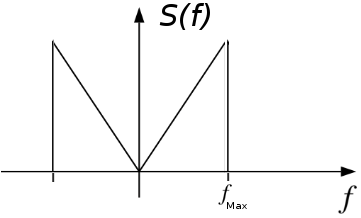
\includegraphics[scale=0.4]{images/fmax.png}
\caption{Spektrum des Signals mit maximaler Frequenz $f_{max}$}
\label{fmax}
\end{figure}

nach dem Abtasten folgendes Spektrum:

\begin{figure}[h!]
\centering
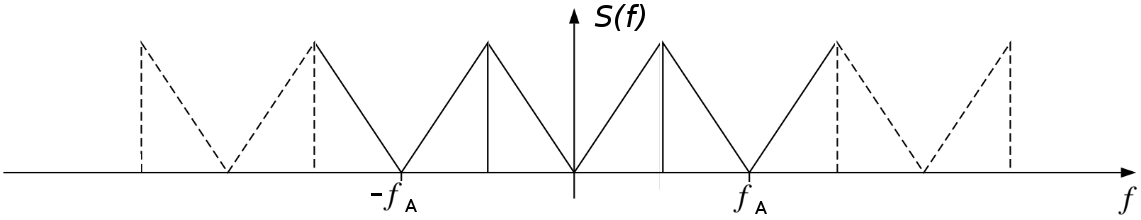
\includegraphics[scale=0.3]{images/2f.png}
\caption{Spektrum des mit $2f_{max}$ abgetasteten Signals.}
\label{2fsig}
\end{figure}
\newpage

Es ist offensichtlich, dass sich die periodischen Frequenzbänder an der Stelle $n \cdot f_A$ berühren, und ein einzelnes Band an dieser Stelle somit nicht eindeutig rekonstruiert werden kann. Wird eine geringere Abtastfrequenz gewählt, so überschneiden sich die Frequenzbänder, und das so genannte 'Aliasing' betrifft größere Bereiche des Signals. Aliasing ist irreversibel und sollte somit vermieden werden.

\subsubsection{Reale Abtastung}

Gegeben sei das abgetastete Signal\\
$$s_{AW}(t) = rect\left(\frac{t}{T_W}\right) * \sum_{n=-\infty}^{\infty} s(t) \delta (t - n\cdot T_A)$$\\
Die Fouriertransformation ergibt das folgende Spektrum:\\
\begin{equation}
\begin{aligned}
\mathcal{F}(s_{AW}(t)) = &  \mathcal{F}(rect\left(\frac{t}{T_W}\right) * \sum_{n=-\infty}^{\infty} s(t) \delta (t - n\cdot T_A)) \\
= & \mathcal{F}(rect\left(\frac{t}{T_W}\right)) \cdot \mathcal{F}(\sum_{n=-\infty}^{\infty} s(t) \delta (t - n\cdot T_A)) \\
= & T_W \cdot si(\pi f T_W) \cdot \left[ S(F) * \frac{1}{T_A} 
\sum_{n=-\infty}^{\infty} \delta \left(f - \frac{n}{T_A}\right) \right] \\
\end{aligned}
\end{equation}

Dabei beschreibt $$si(t) = \frac{sin(t)}{(t)}$$

Vergleicht man dieses Ergebnis mit dem Spektrum der idealen Abtastung, so ergibt sich:
$$S_{AW}(f) = T_W \cdot si(\pi f T_W) \cdot S_{a}(f)$$

Dies entspricht dem idealen Spektrum, allerdings durch die eine si-Funktion verzerrt. Dies ist in der Rekonstruktion behandelbar und somit im Gegensatz zu Aliasing reversibel.\\

\subsection{Implementierung eines ADU}
Von zentraler Bedeutung ist die praktische Realisierung einer Abtastschaltung. Neben der Abtastung müssen die Daten jedoch in der Regel in eine digitale Form konvertiert werden, um diese mithilfe eines Computersystems verarbeiten zu können. Der Analog-Digital-Umsetzer (ADU) realisiert diese Konvertierung und kann in vielen Varianten implementiert werden.\\
Im Folgenden wird eine Schaltung vorgestellt, welche aus Abtastung mithilfe einer Abtast-Halte-Schaltung sowie eines Single-Slope-Umsetzers besteht.
\subsubsection{Abtastung}
\label{3.3.1}

\begin{figure}[h!]
\centering
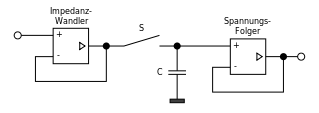
\includegraphics[scale=0.8]{images/abtastung_schaltung.png}
\captionsource{Schematische Anordnung eines Abtast-Halte-Gliedes}{\cite{sah_schaltung}}
\label{sah_schaltung}
\end{figure}

Zunächst wird das eingehende Signal auf einen Impedanzwandler gegeben, welcher die Impedanz der Quelle der des Verbrauchers anpasst. Dies verhindert eine zu hohe Belastung der Spannungsquelle, wodurch gegebenenfalls Ungenauigkeiten in der Messung auftreten können.\\
Die Rückkopplung des Impedanzwandlers ist durch einen Schalter mit einem Kondensator parallel zu einem Spannnungsfolger verbunden. Wird dieser geschlossen, so lädt sich während des Zeitfensters $T_W$ der Kondensator mit der eingehenden Spannung auf. Währenddessen ist es möglich, dass sich die Spannung verändert. Anschließend wird der Schalter wieder geöffnet, und somit ist die auf der rechten Seite der Schaltung anliegende Spannung konstant, da diese durch den Kondensator gespeichert wird. Der Spannungsfolger wird eingebaut, um die Spannung möglichst lange zu halten, damit der ausgehende Wert als konstant angenommen werden kann.\\

Der gesamte ADU könnte auch ohne diese Schaltung implementiert werden. Im Folgenden wird jedoch erläutert, weshalb sie für nicht konstante Eingangsspannungen sehr anfällig ist, weswegen die	Wandlung eines zeitkontinuierlichen- in ein zeitdiskretes Signal eingebunden wird.

\subsubsection{Single-Slope-Umsetzer}

Nach erfolgreicher Abtastung liegt ein Signal in zeitdiskreter Form vor. Der zugehörige Wert für jedes Zeitfenster $T_W$ kann als annähernd konstant angenommen werden, sofern die Fensterbreite nicht zu groß ist und der Spannungsfolger die Spannung nahezu verlustlos halten kann. Anschließend folgt die Übersetzung in ein digitales Signal. Hierfür existieren eine Vielzahl an Verfahren, wobei im Folgenden ein vergleichsweise Einfaches vorgestellt wird, um den Vorgang zu verdeutlichen.

\begin{figure}[h!]
\centering
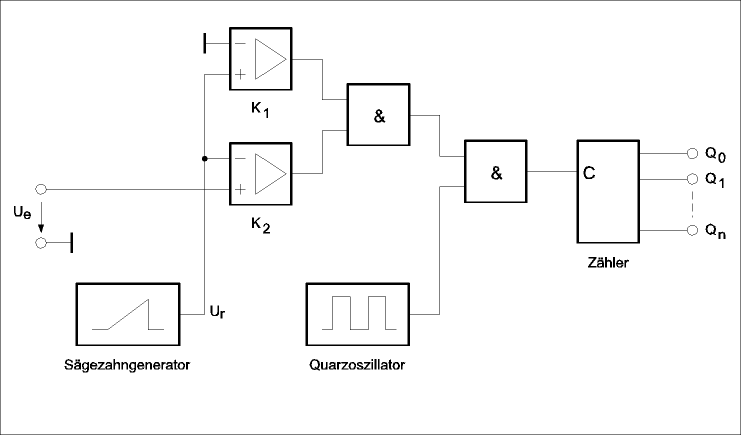
\includegraphics[scale=0.4]{images/singleslope.png}
\captionsource{Schematische Anordnung eines Single-Slope-Umsetzers}{\cite{singleslope_schaltung}}
\label{singleslope_schaltung}
\end{figure}

\ref{singleslope_schaltung} zeigt den Aufbau solch einer Schaltung. Zunächst wird eine Sägezahnspannung erstellt, welche mittels zwei Komparatoren mit der Eingangsspannung- sowie des Massepotentials verglichen wird. Der Vergleich mit dem M	assepotential dient dazu, dass das Signal nur während einer Flanke der Sägezahnspannung gemessen wird. Solange diese Spannung größer als die 'konstante' Eingangsspannung ist, schaltet das erste (linke) \&-Gatter. Währenddessen erstellt der Quarzoszillator ein periodisches Rechtecksignal, dessen Periode nur einen Bruchteil der Steigungsdauer der Sägezahnspannung entspricht. Bei jeder Periode schaltet das zweite \&-Gatter, und der Zähler bekommt einen Impuls. Sobald die Sägezahnspannung gleich der Eingangsspannung ist, wird der Zähler nicht mehr inkrementiert. Jeder Flanke des Oszillators wird eine Spannung $dU$ zugeordnet, mit 
$$dU = max(U_r) \cdot \frac{f_{Oszi}}{f_r}$$\\
wobei $f_{Oszi}$ die Frequenz des Oszillators, $f_r$ die Frequenz der Sägezahnspannung und $U_r$ den maximalen Wert der Sägezahnspannung beschreibt.\\
Wurden am Zähler $n$ Flanken gezählt, so liegt die Spannung $n \cdot dU$ in digitaler Form am Ausgang des Zählers vor. Dabei ist offensichtlich, dass diese Spannung nur einen Wert $k \cdot dU, k \in R$ annehmen kann. Wird die Anzahl an Ausgabebits des 	Zählers erhöht, so können eingehende Flanken in höherer Frequenz verarbeitet werden, da die 'Auflösung' des Zählers gestiegen ist.\\
Weiterhin muss beachtet werden, dass eine höhere Abtastfrequenz eine im gleichen Maße höhere Frequenz des Oszillators- und des Sägezahngenerators erfordert. Wird die Frequenz des Oszillators nicht angepasst, so sinkt die Auflösung des Zählers, da auf eine Periode der Sägezahnspannung nun weniger Messperioden folgen.\\

Dieses Verfahren bietet eine vergleichsweise einfache, dafür jedoch sehr limitierte Lösung. Neben der maximslen Taktfrequenz des Oszillators, welche bei hoher Auflösung leicht erreicht wird schränkt auch die Instabilität gegenüber nicht konstanten Eingangsspannungen das System ein. In Verbindung mit des in \ref{3.3.1} vorgestellten Abtast-Halte-Glieds ist dieser Aufbau für Grundlegende Problemstellungen jedoch ausreichend.

\subsection{Bedeutung}\label{3.3}

Nach der Abtastung eines Signals liegt dies zwangsweise in diskreter Form vor, sowohl im zeit- als auch im Wertebereich. Dies hat mehrere Ursachen. Zum einen existieren keine Messinstrumente, welche eine beliebige Größe beliebig genau messen können. So existieren beispielsweise High-End Sensoren, welche Temperaturen mit einer Auflösung von $\pm0.125^\circ C$ messen können und einer Genauigkeit von $\pm0.1^\circ C$ erfassen können. Es ist absehbar, dass diese Werte in Zukunft verbessert werden können, also Temperaturen genauer und mit einer geringeren Unsicherheit erfasst werden können. Jedoch zeigt sich auch, dass der praktischen Messung Grenzen gesetzt sind.\\
Die andere Problematik entspringt aus Speicherung gemessener Daten. Man nehme an, es existiere ein Messinstrument, welches beispielsweise Spannung beliebig genau messen könnte, und dies in beliebigen Zeitabständen. Wird nun eine Spannung gemessen und mit einer Genauigkeit von 15 Dezimalstellen gemessen, und dies geschieht mit einer Frequenz von $1M$Hz, so fallen $1 \cdot 10^6 \cdot 64$ bit $= 64 \cdot 10^6$ bit $= 8M$B an Informationen die Sekunde an. Dies wird auch als Datenrate bezeichnet.\\
In dem Fall mit einer beliebig großen Genauigkeit - sowie Frequenz ist dieser Datenrate keine Grenze gesetzt. Neben der offensichtlichen Problematik der Speicherung wird auch die Übertragung der Daten von ADU zu Prozessor und Speichereinheit ein bedenklicher Aspekt, welcher eben diese Datenrate limitiert.

\subsection{Periphere Schnittstellen}\label{3.4}
\subsection{Analoger und digitaler In-/Output}\label{3.5}